\section{Мета роботи}
набути навичок та закріпити знання при виконанні операцій на
мультисписках та нелінійних списках.
\\

\noindent
\textbf{Теми для попередньої роботи:}
\begin{itemize}
    \item набори даних – списки: лінійні, кільцеві, мультисписки, нелінійні списки;
    \item операції на списках.
\end{itemize}



\section{Завдання}
Для варіантів завдань 1 – 13 розробити програму, що створює список
списків (нелінійний список). Передбачити такі функції:
\begin{itemize}
    \item додавання елементів у список та підсписок (при додаванні елемента у головний список додається і відповідний підсписок);
    \item видалення елементів зі списку та підсписків (при видаленні елемента з головного списку видаляється і пов’язаний з ним підсписок);
    \item видача вмісту списків та підсписків у консоль;
    \item видалення списків.
\end{itemize}
Завдання обрати у табл. 8.1 згідно зі своїм номером у журналі групи.

\begin{figure}[ht!]
    \centering
    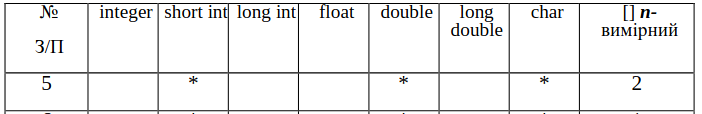
\includegraphics[width=.9\textwidth]{\assetsDirectory/var.png}
    \caption{Завдання за варіантом (\variant)}
\end{figure}



\section{Хід виконання}
Для виконання завдання було обрано мову Rust.
Увесь код також додатково був розміщений в GitHub репозитарії: \href{https://github.com/blackgolyb/algos-labs}{https://github.com/blackgolyb/algos-labs}.


\newpage
\subsection{Non linear list}
Зробимо його елемент таким, що в ньому можуть лежати такий же non linear list та якийсь значення.
Таким чином ми можемо побудувати структуру будь-якої ієрархії та при цьому зберігати значення.
Для взаємодії з списком ми реалізуємо такі функції:

\begin{itemize}
    \item Додання елемента. Якщо такої вкладеності ще нема, то вона автоматично створиться.
    \item Додання підсписку. Якщо такої вкладеності ще нема, то вона автоматично створиться.
    \item Видалення елемента / підсписка.
    \item Взяття елемента / підсписка.
    \item Вивід на екран.
\end{itemize}

\lstinputlisting[language=Rust, style=colouredRust]{\codeDirectory/src/libs/list/non_linear_list.rs}


\newpage
\subsection{Приклад роботи програми}
Для перевірки працездатності напишемо програму яка буде автоматично генерувати значення для списків.
Потім виконаємо наступні дії та виведемо обидві версії на екран для порівняння, а також виділемо зміни елементи:

\begin{enumerate}
    \item Додамо два елементи у за такими індексами [2, 2, 2] та потім [2, 2, 0].
    Таким чином перевіримо автоматичне додання підсписка та додання елементів.
    \item Видалимо список за індексом [6]
    \item Видалимо значення за індексом [7]
    \item Видалимо значення та список за індексом [8]
\end{enumerate}


\noindent
Код програми для перевірки:
\lstinputlisting[language=Rust, style=colouredRust]{\codeDirectory/src/labs/lab8/main.rs}

\begin{figure}[ht!]
    \centering
    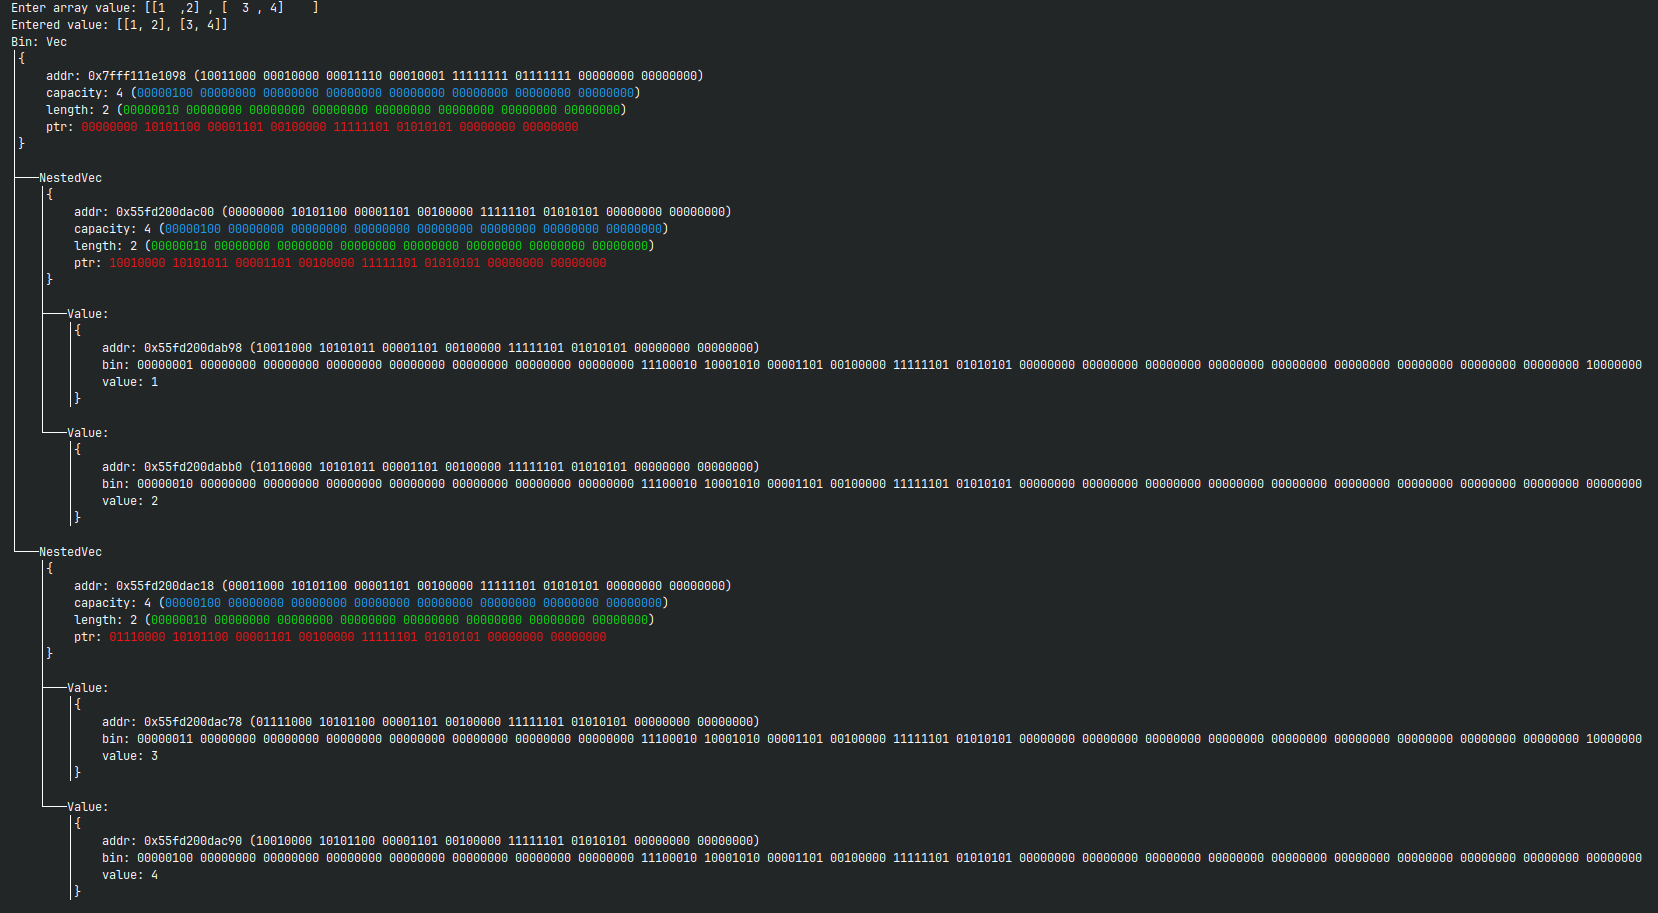
\includegraphics[width=\textwidth]{\assetsDirectory/res.png}
    \caption{Приклад роботи}
\end{figure}


\newpage
\section{Висновки}
В ході виконання лабораторної робити було створено нелінійний список на базі двозв'язного списку.
